\documentclass[12pt]{article}
\usepackage[margin = 1in]{geometry}
\usepackage{amsmath}
\usepackage{amssymb}
\usepackage{amsthm}
\usepackage{graphicx}
\usepackage{subfig}
\usepackage{enumitem}

\begin{document}
	
	\begin{center}
		\textbf{Quiz 11} \\
		\textbf{Differential Equations} \\
		\textbf{Math 337} \\
		\textbf{Stephen Giang} \\
	\end{center}

\noindent \textbf{Problem 1: }Consider the periodic function $f(t)$ defined as follows:
	$$
	f(t) = 
	\begin{cases}
		t,  & 0 \leq t < 2 \\
		4-t, & 2\leq t < 4
	\end{cases},
	\qquad \text{with} \qquad 
	f(t+4) = f(t)
	$$
Sketch a graph of this function for $t \in [0, 12]$. Write this function as a window function, $f_4(t)$, (Slide 22) using step functions. Use our Theorem (Slide 23) to obtain the Laplace Transform, $\mathcal{L}[f(t)] = F(s)$. This expression simplifies by dividing out a common factor in the numerator and denominator. Follow the example in the Lecture Slides to express the resulting rational expression in terms of a geometric series.
	\begin{figure}[h]
		\centering
		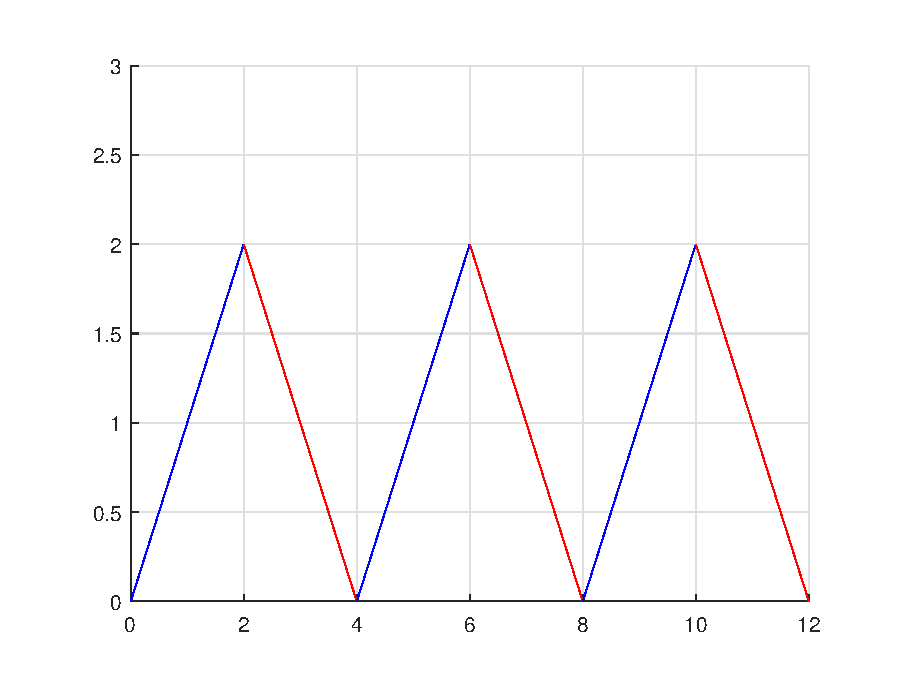
\includegraphics[width = 10cm,height = 4cm]{Prob1f4}
	\end{figure}
	\begin{align*}
		f_4(t) &= t[u_0(t) - u_2(t)] + (4-t)[u_2(t) - u_4(t)] \\
		&= tu_0(t) - tu_2(t) + 4u_2(t) - tu_2(t) + (t-4)u_4(t) \\
		&= t - 2(t - 2)u_2(t) + (t-4)u_4(t)
	\end{align*}
	\begin{align*}
		\mathcal{L}[f(t)] &= \frac{1}{1 - e^{-4s}}\mathcal{L}[f_4(t)] \\
		&= \frac{1}{1 - e^{-4s}}\left(\frac{1}{s^2} - \frac{2e^{-2s}}{s^2} + \frac{e^{-4s}}{s^2}\right) \\
		&= \frac{1}{1 - e^{-4s}}\left(\frac{e^{-4s} - 2e^{-2s} + 1}{s^2}\right) \\
		&= \frac{1}{(1 - e^{-2s})(1 + e^{-2s}) }\left(\frac{(1 - e^{-2s})^2}{s^2}\right) \\
		&= \frac{1 - e^{-2s}}{s^2} \left(\frac{1}{1 + e^{-2s}}\right) \\
		&= \frac{1 - e^{-2s}}{s^2}\left(1 - e^{-2s} + e^{-4s} + ... + (-1)^ne^{-2ns}\right) \\
		&= \frac{1 - e^{-2s}}{s^2}\sum_{n = 0}^{\infty} (-1)^ne^{-2ns}
	\end{align*}

\newpage 

\noindent \textbf{Problem 2: }Solve the following initial value problem with Laplace transforms:
	$$
	y' + 4y = f(t), \qquad y(0) = 2
	$$
where $f(t)$ is the periodic function given in the previous problem above. Show all the steps needed
to find $\mathcal{L}[y(t)] = Y(s)$, then show the necessary partial fractions decomposition (PFD) required to
make your elements appear in the Laplace table. Finally, invert Y (s) to find your solution
\\ \\
Notice the following:
	\begin{align*}
		\mathcal{L}[y' + 4y] &= sY(s) - y(0) + 4Y(s) = \frac{1 - e^{-2s}}{s^2}\sum_{n = 0}^{\infty} (-1)^ne^{-2ns} \\
		&= (s+4)Y(s) - 2 = \frac{1 - e^{-2s}}{s^2}\sum_{n = 0}^{\infty} (-1)^ne^{-2ns}
	\end{align*}
Notice the partial fractions decomposition:
	\begin{align*}
		\frac{1}{s^2(s+4)} &= \frac{A}{s} + \frac{B}{s^2} + \frac{C}{s+4} \\
		1 &= (A+C)s^2 + (4A+B)s + 4B
	\end{align*}
So we get $B = \frac{1}{4}$, $A = \frac{-1}{16}$, and $C = \frac{1}{16}$
	\begin{align*}
		Y(s) &= \frac{2}{s+4} + \left(\frac{-1}{16s} + \frac{1}{4s^2} + \frac{1}{16(s+4)}\right)\left(1 - e^{-2s}\right)\sum_{n = 0}^{\infty} (-1)^ne^{-2ns} \\
		&= \frac{2}{s+4} + \left(\frac{-1}{16s} + \frac{1}{4s^2} + \frac{1}{16(s+4)}\right)\left(1 - e^{-2s}\right)\sum_{n = 0}^{\infty} (-1)^ne^{-2ns} \\
		y(t) &= 2e^{-4t} + \left(\frac{-1}{16} + \frac{t}{4} + \frac{e^{-4t}}{16}\right)(1 - u_2(t)) + \sum_{n = 1}^{\infty} (-1)^nu_k(t)\left(\frac{-1}{16} + \frac{t}{4} + \frac{e^{-4t}}{16}\right)
	\end{align*}

\newpage 

\noindent \textbf{Problem 3: }Solve the following initial value problem with Laplace transforms:
	$$
	y'' + 4y' + 5y = \frac{2t}{\pi}(\delta(t-\pi) - \delta(t-2\pi)), \qquad y(0) = 0, \quad y'(0) = 2 
	$$
Use the Laplace table to find your solution. Use the computer to create a graph of your solution
for $t \in [0, 15]$. What is the limiting solution for large t?
\\ \\
Notice the following:
	\begin{align*}
		\mathcal{L}\left[\frac{2t}{\pi}(\delta(t-\pi) - \delta(t-2\pi))\right] &= 2\mathcal{L}\left[\frac{t}{\pi}\delta(t-\pi)\right] - 4\mathcal{L}\left[\frac{t}{2\pi}\delta(t-2\pi)\right] \\
		&= 2e^{-\pi s} - 4e^{-2\pi s} \\ \\
		\mathcal{L}\left[y'' + 4y' + 5y\right] &= s^2Y(s) - sy(0) - y'(0) + 4sY(s) - 4y(0) + 5Y(s) \\
		&=(s^2 + 4s + 5)Y(s) - 2  
		\\ \\
		Y(s) &= \frac{2}{(s+2)^2 + 1} + \frac{2e^{-\pi s}}{(s+2)^2 + 1} - \frac{4e^{-2\pi s}}{(s+2)^2 + 1} 
		\\ \\
		y(t) &= 2e^{-2t}\sin(t) + 2u_\pi(t)e^{-2(t-\pi)}\sin(t - \pi) - 4u_{2\pi}(t)e^{-2(t-2\pi)}\sin(t - 2\pi)
	\end{align*}
The limiting solution:
	$$
	\lim\limits_{t \rightarrow \infty} y(t) = 0
	$$
	\begin{figure}[h]
	\centering
	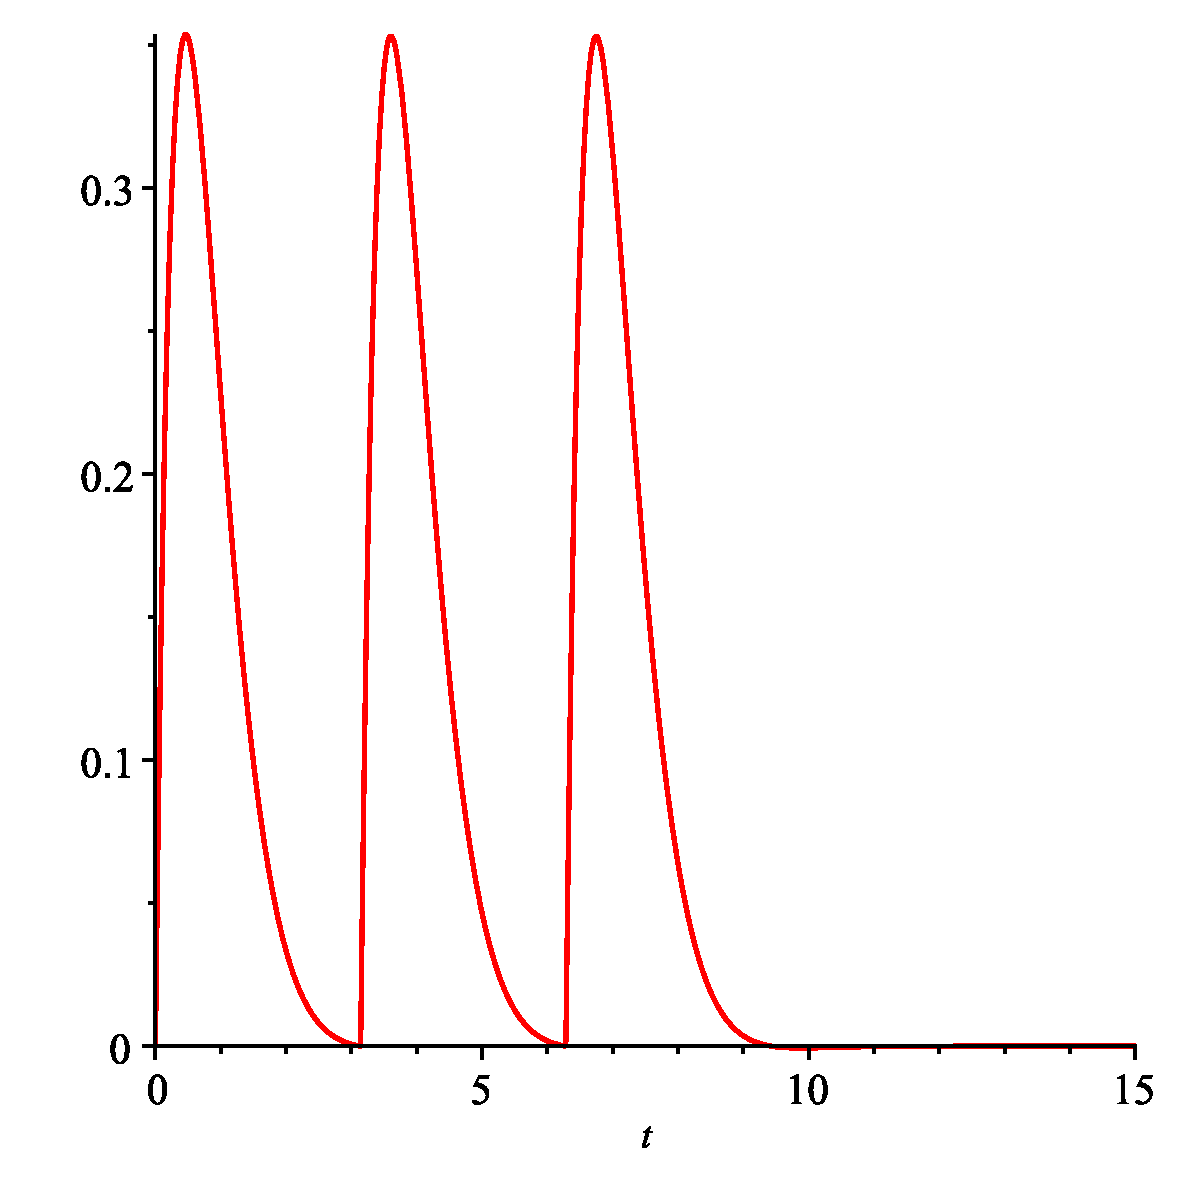
\includegraphics[width = 10cm, height = 6cm]{Prob3}
	\end{figure}
	
	
	
	
	
	
	
	
	
	
	
	
	
	
	
	
	
	
	
	
	
	
\end{document}
